% !TeX spellcheck = ru_RU-Russian

\documentclass{beamer}
\mode<presentation>
\usetheme{Ilmenau}

\usepackage[utf8]{inputenc}
\usepackage[T1,T2A]{fontenc}
\usepackage{hyperref}
\hypersetup{colorlinks=true}
\usepackage{tikz}
\usetikzlibrary{fit}

\def \MinSize {22}

\newcommand{\mtx}[1]{\boldsymbol{#1}}

\tikzstyle{fcnode}=[
  thick,
  draw=black,
  rectangle,
  minimum height=2*\MinSize,
  minimum width=1.5*\MinSize
]

\tikzstyle{neuron}=[
  draw=black,
  circle,
  minimum size=\MinSize
]

\begin{document}

\section{Модель нейрона}

\begin{frame}
  \begin{columns}

    \begin{column}{0.5\textwidth}
      $$ y = \sum_{i}^{} w_i \cdot x_i + b $$
    \end{column}

    \begin{column}{0.5\textwidth}
      \begin{center}
        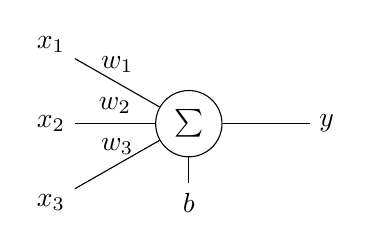
\begin{tikzpicture}
          \def \x {3}
          \def \y {0}
          \def \xOff {1.75}
          \def \yOff {1}

          \node[neuron] (n1) at (\x, \y) {$\sum$};

          % ins
          \node (x1) at (\x - \xOff, \y + \yOff) {$x_1$};
          \node (x2) at (\x - \xOff, \y) {$x_2$};
          \node (x3) at (\x - \xOff, \y - \yOff) {$x_3$};
          \node (b1) at (\x, \y - \yOff) {$b$};

          % out
          \node (y1) at (\x + \xOff, \y) {$y$};

          % connect ins
          \foreach \i in {1,...,3}{
            \draw (x\i) -- (n1) node[midway,above] {$w_\i$};
          }
          \draw (b1) -- (n1);

          % connect out
          \draw (n1) -- (y1);
        \end{tikzpicture}
      \end{center}
    \end{column}

  \end{columns}
\end{frame}

\section{Линейный слой}

\begin{frame}{\secname : \subsecname}
  \framesubtitle{Полносвязный слой, fully connected, linear}
  \begin{columns}

    \begin{column}{0.5\textwidth}
      Здесь и далее используются обозначения, принятые в PyTorch:
      $$
      y = x \cdot \mtx{A}^T + b
      $$
      где $\mtx{A}[O \times I]$~--- матрица обучаемых весов,
      подробнее в
      \href{https://docs.pytorch.org/docs/stable/generated/torch.nn.Linear.html}{документации}

    \end{column}

    \begin{column}{0.5\textwidth}
      \begin{center}
        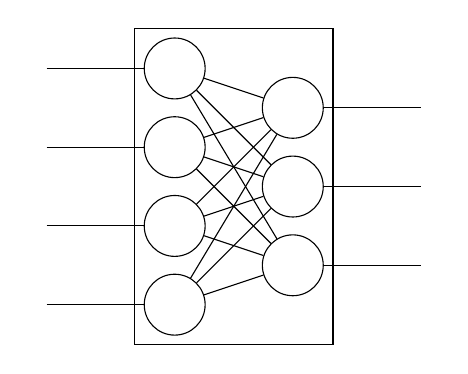
\begin{tikzpicture}
          \def \InSize {3}
          \def \OutSize {2}

          \def \OffX {1.75}

          \def \InX {0}
          \def \InY {-3}
          \def \OffInY {1}

          \def \OutX {1.5}
          \def \OutY {-2.5}
          \def \OffOutY {1}

          \foreach \i in {0,...,\InSize}{
            \def \y {\InY + \i * \OffInY}
            \node[neuron] (n\i) at (\InX, \y) {};
            \node (x\i) at (\InX - \OffX, \y) {};
            \draw (x\i) -- (n\i);
          }

          \foreach \i in {0,...,\OutSize}{
            \def \y {\OutY + \i * \OffOutY}
            \node[neuron] (m\i) at (\OutX, \y) {};
            \node (z\i) at (\OutX + \OffX, \y) {};
            \draw (z\i) -- (m\i);
          }

          \foreach \i in {0,...,\InSize}{
            \foreach \j in {0,...,\OutSize}{
              \draw (n\i) -- (m\j);
            }
          }

          \node[draw, fit=(n0) (n\InSize) (m0) (m\OutSize)] {};
        \end{tikzpicture}
      \end{center}
    \end{column}

  \end{columns}
\end{frame}

\begin{frame}

\end{frame}

\section{Введение}

\section{Перцептрон}

\section{Функция активации}

\end{document}
